% =====================================================================================
% begin PREAMBLE
% =====================================================================================
\documentclass[a4paper, 11pt]{article}

% =====================================================================================
% PACKAGES
% =====================================================================================
\usepackage{amssymb,amsfonts,amsmath}
\usepackage{graphics}
\usepackage[dvips]{graphicx}
\usepackage{color}
\usepackage[usenames, dvipsnames]{xcolor}
\usepackage{subfigure}
\usepackage{mathtools}
\usepackage[normalem]{ulem}
\usepackage{dcolumn}
\usepackage{multirow}
\usepackage{booktabs}
\usepackage{bm}
\usepackage{fullpage}
\usepackage{mathrsfs}
% \usepackage{showkeys}
\usepackage{cancel}
% \usepackage{xfrac}
\usepackage[linktocpage,colorlinks=true,linkcolor=blue,citecolor=blue]{hyperref}

% =====================================================================================
% DEFINE NEW COMMANDS
% =====================================================================================
% Editorial
\newcommand{\note}[1]{(\emph{\color{blue}{#1}})}
\newcommand{\edit}[1]{{\color{blue}{#1}}}
\newcommand{\change}[2]{{\color{red}\sout{#1}}{\color{blue}\emph{#2}}}
\newcommand{\faded}[1]{{\color{gray} #1}}
% Mathematical
\newcommand{\mf}[1]{\ensuremath{\mathbf{#1}}}
\newcommand{\la}{\langle}
\newcommand{\ra}{\rangle}
\newcommand{\nrm}{\ensuremath{\mathcal{M}} }
\newcommand{\mrm}[1]{\ensuremath{\mathrm{#1}}}
\newcommand{\cond}{\ensuremath{\, | \,}}
\newcommand{\conds}[2]{\ensuremath{#1 \!\cond\! #2}}
% SPECIFIC TO FILE
\newcommand{\ovb}[2]{\ensuremath{\overbracket[0.5pt]{\widehat{\mf{\, #1}}^{(\, #2)}}}}
\newcommand{\unv}[1]{\ensuremath{\hat{\mf{#1}}}}
\newcommand{\exhat}{\ensuremath{\mf{\widehat{e}_x}}}
\newcommand{\eyhat}{\ensuremath{\mf{\widehat{e}_y}}}
\newcommand{\ezhat}{\ensuremath{\mf{\widehat{e}_z}}}
% COLOURS AND LINKS
\definecolor{royalblue}{rgb}{0,0.08,0.45}
% =====================================================================================
% end PREAMBLE
% =====================================================================================

% =====================================================================================
%  TITLE 
% =====================================================================================
\title{\textsf{\Huge IISERK-IMSc Hydrodynamic Collaboration \\ Plan of Action}}

% =====================================================================================
% AUTHORS, AFFILIATIONS 
% =====================================================================================
\author
  {\textsf{Basudev Roy, Ayan Banerjee} \\ \\
   \textsc{Indian Institute of Science Education and Research,} \\
   \textsc{Kolkata 700064, India} \\ \\ \\
   \textsf{Somdeb Ghose, R. Adhikari} \\ \\
   \textsc{The Institute of Mathematical Sciences,} \\
   \textsc{CIT Campus, Chennai 600113, India} 
  }

% ===================== DATE ==========================================================
% \date{April 1, 2012}
\date{\today}

% =====================================================================================
% begin DOCUMENT
% =====================================================================================
\begin{document}

% ===================== MAKETITLE =====================================================
\maketitle

% =====================================================================================
% ABSTRACT 
% =====================================================================================
\begin{abstract}
Lorem ipsum dolor sit amet
\end{abstract}

\newpage
% =====================================================================================
\section{Hydrodynamic interactions between passive spherical particles in an optical trap}
% =====================================================================================

\subsection{Experimental setup}

% ============================================================================================
% FIGURE #
% ============================================================================================
\begin{figure}[h!]
\begin{center}
    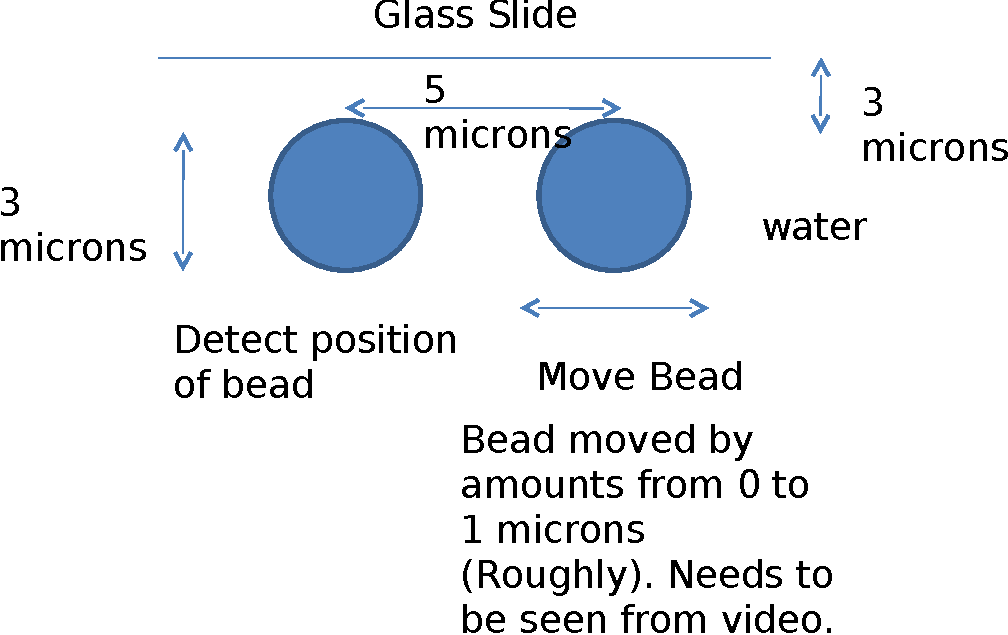
\includegraphics[width=0.80\textwidth]{HI_setup}
%     
  \caption{ Experimental setup.
  \label{fig:expt_setup_two_spheres}}
\end{center}
\end{figure}
% ============================================================================================

\subsection{Results}

Basudev Roy :

\begin{quotation}
These 4 files are the displacement of the test bead in the presence of the first bead which has been excited by a square wave pulse. The first bead moves as an exponential between the two positions. We pick the displacement of the test bead located in a shallow trap in the presence of the first bead. The displacement is recorded with a quadrant photodiode and has a unit of Volts which is proportional to the actual displacement. Each data set has been averaged over 38 subsequent times the experiment is repeated. Please note that 250 ms of data corresponds to two square wave pulses. The phase delay between the initial square wave and this particular response has not been recorded. 

We could record the time constant of the decaying exponential motion of the first bead in a later experiment. We can do a much more elaborate 
experiment about the coupling if you could match these trajectories first. If it doesnt match at all, we know there is a problem with the 
way the experiment has been performed in the first place. 

The distance between the centers of the beads is 4 microns and the diameter is 3 microns. 

The displacements of the first bead are represented in Volts in terms of the amplitude of the square wave that drives the accousto optic modulator.
The separation between the equilibrium spots of the bead is proportional to this voltage.   
\end{quotation}

% ============================================================================================
% FIGURE #
% ============================================================================================
\begin{figure}[h!]
\begin{center}
    \subfigure[]{ 
    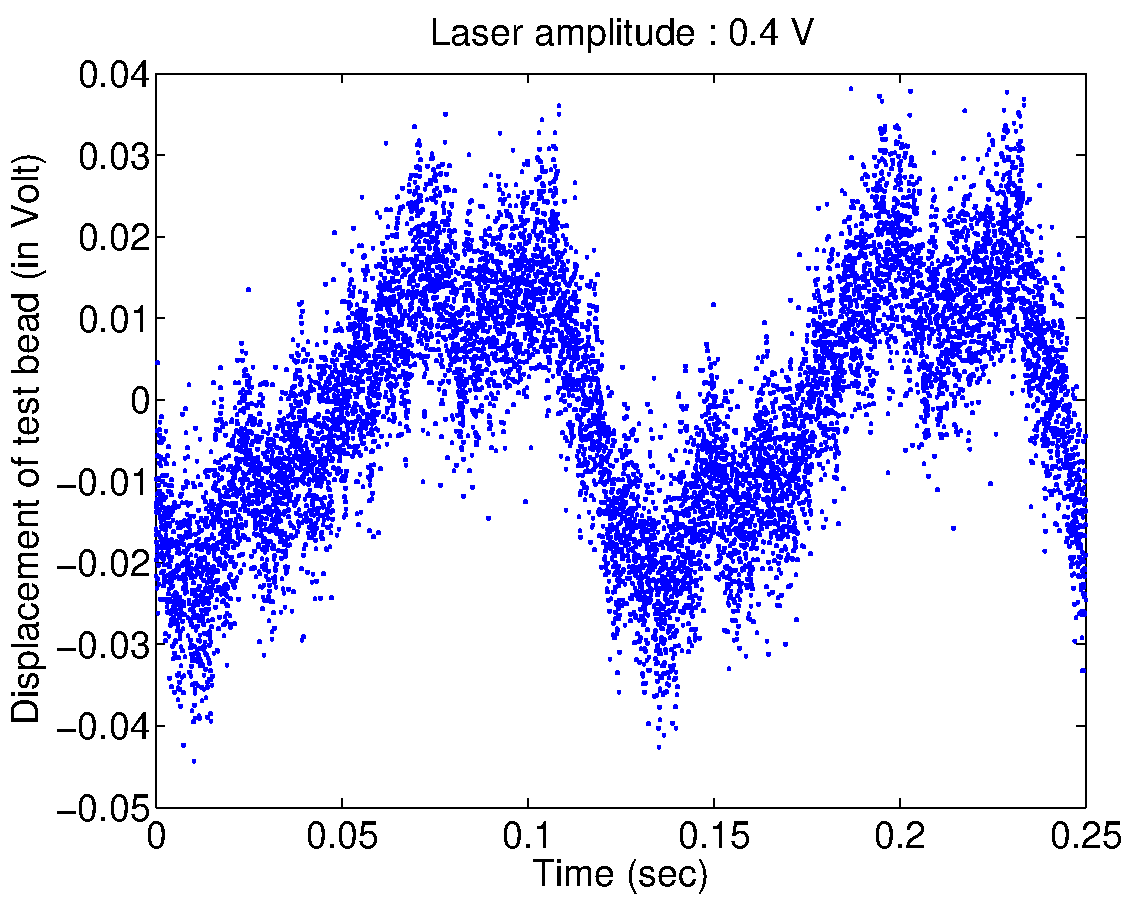
\includegraphics[width=0.45\textwidth]{hyd_interact_4_0dot4} 
    \label{fig:hyd_interact_4_0dot4}}
    \subfigure[]{ 
    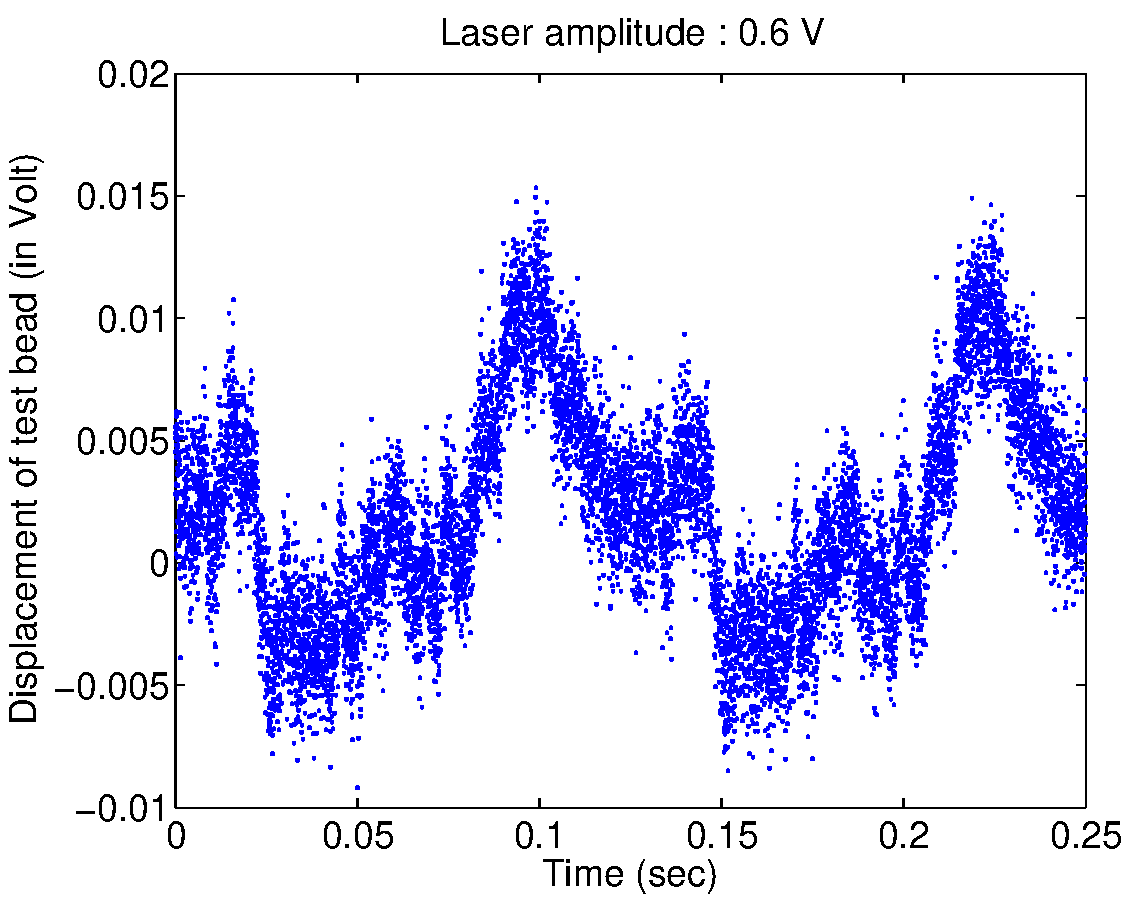
\includegraphics[width=0.45\textwidth]{hyd_interact_4_0dot6} 
    \label{fig:hyd_interact_4_0dot6}} 
    \\
    \subfigure[]{ 
    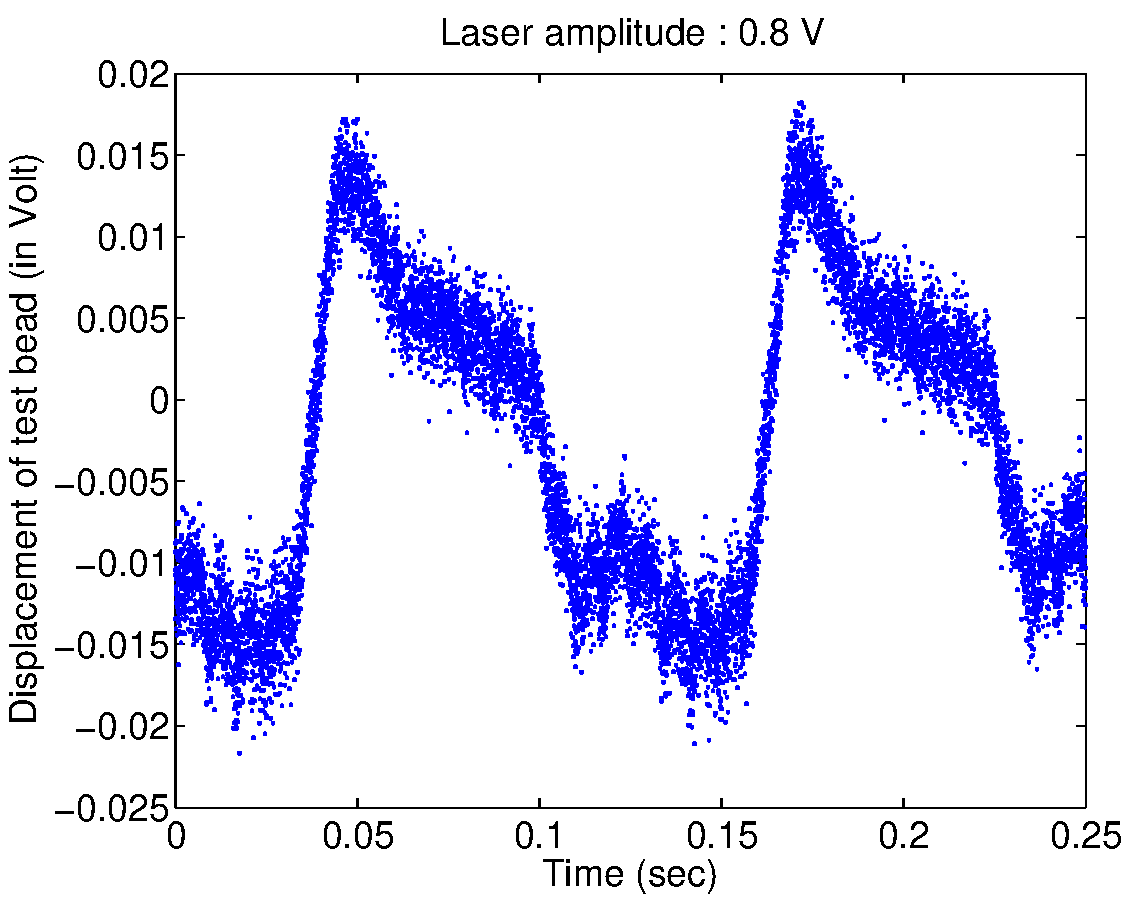
\includegraphics[width=0.45\textwidth]{hyd_interact_4_0dot8} 
    \label{fig:hyd_interact_4_0dot8}}
    \subfigure[]{ 
    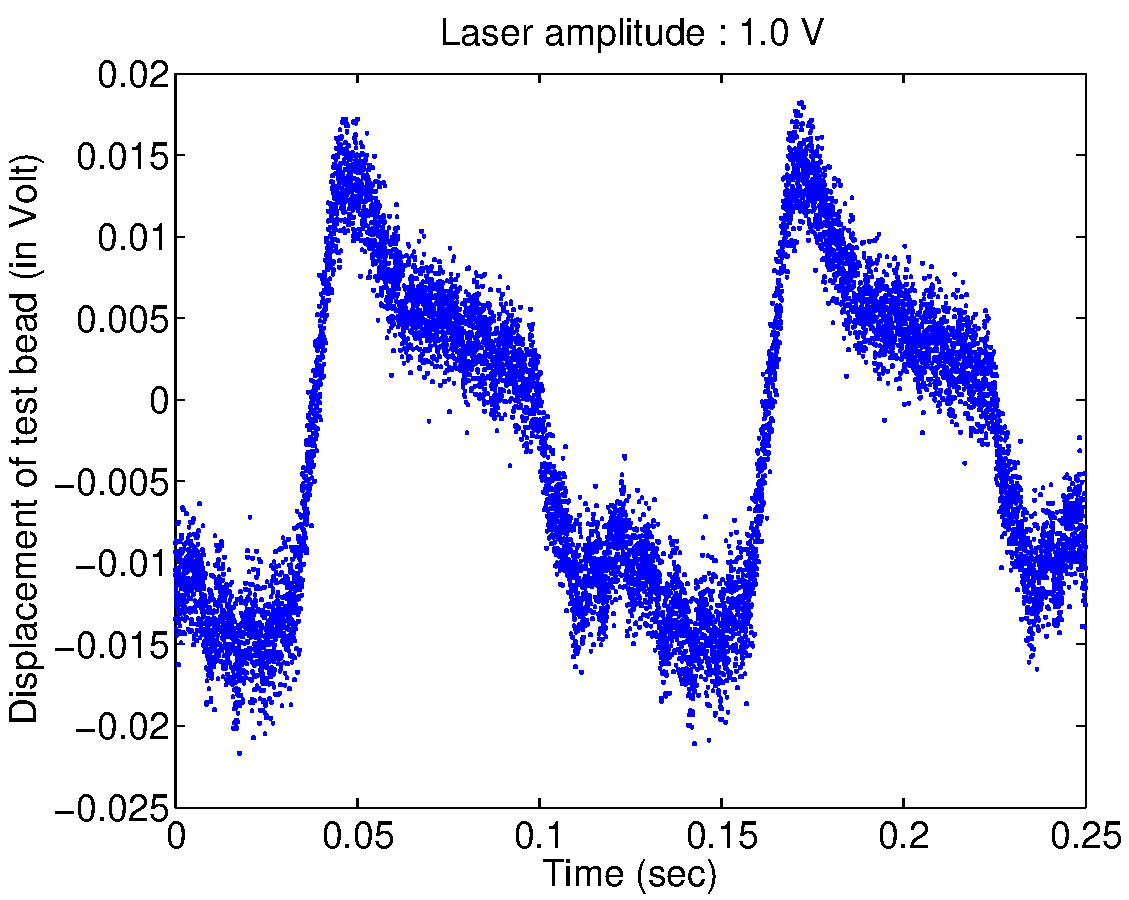
\includegraphics[width=0.45\textwidth]{hyd_interact_4_1dot0} 
    \label{fig:hyd_interact_4_1dot0}}
%     
  \caption{ Displacement of the test bead in the presence of the first bead which has been excited by a square wave pulse.
  \label{fig:two_spheres_response}}
\end{center}
\end{figure}
% ============================================================================================

\subsection{Theory}

Ronojoy Adhikari , addressing AB and BR :

\begin{quotation}
  Four possible situations you can have for the hydrodynamic interactions in this situation:

  \begin{enumerate}
    \item Two particles in an infinite fluid - the boundaries are many particle radii away from the particle centers.
    \item Two particles in a semi-infinite fluid - at least one boundary is several particle radii away from the particle centres
    \item Two particles in a bounded fluid - more than one boundary is several particle radii away from the particle centers
    \item Particles at a phase boundary
  \end{enumerate}

It seems that you have situation (2), but, if you reduce the width of your setup, you might end up in situation (3). Theoretically, (1), (2), (3) and (4) are in increasing order of difficulty to compute. 
\end{quotation}


\newpage
% =====================================================================================
\section{Nucleation and growth of bubbles in a laser-heated optical trap}
% =====================================================================================

% =====================================================================================
\section{Nucleation and growth of anisotropic bubbles in a nematic domain in a laser-heated optical trap}
% =====================================================================================

\[ 
  \alpha ~ \beta ~ \gamma ~ \delta ~ \mu ~ \nu ~ +
\]



% =====================================================================================
% BIBLIOGRAPHY
% =====================================================================================
\bibliographystyle{siam}
% \bibliography{path+filename}
% Sample below:
% \bibliography{/home/somdeb/Dropbox/Share/POL2012/filament}
% =====================================================================================

% =====================================================================================
% % BIBLIOGRAPHY (OUTPUT OF .BBL)
% =====================================================================================


% ================== Th-th-that's all, folks! ==================================
\end{document}
